\section{Spazio-tempo delle fasi e struttura di Poisson in tale spazio}
\setcounter{equation}{0}

Consideriamo ora lo spazio $ \mathcal{V}_{n+1} $, che identifichiamo con la varietà $ M $ delle pagine precedenti, e il corrispondente spazio cotangente $ T^* (\mathcal{V}_{n+1}) $. \\
Identifichiamo le coordinate nel modo seguente

\begin{center}
$$ x^1, \dots , x^m \equiv t, q^1, \dots , q^m \qquad \text{in $ \mathcal{V}_{n+1} $} $$
$$ x^1, \dots , x^m , y_1, \dots , y_m \equiv t, q^1, \dots , q^m, P_0, P_1, \dots , P_m \qquad \text{in $ T^* (\mathcal{V}_{n+1}) $} $$
\end{center}

Un elemento di $T^* (\mathcal{V}_{n+1})$ sarà una $ 1 $-forma differenziale rappresentata nella forma

\begin{equation*}
\omega = P_0 (\omega) (dt)_{\pi (\omega)} + P_i (\omega) (dq^i)_{\pi (\omega)}
\end{equation*}
le leggi di trasformazione tra coordinate naturali in $T^* (\mathcal{V}_{n+1})$ avranno la forma
\begin{equation*}
\begin{split}
& t' = t \\
& q'^i = q'^i (t, q) \qquad \leftrightarrow q^i = q^i (t, q'^1, \dots , q'^n) \\
& P'_0 = P_0 + \frac{\partial q^r}{\partial t} P_r \\
& P'_i = P_r \frac{\partial q^r}{\partial q'^i} \\
\end{split}
\end{equation*}

La trasformazione di Liouville su $T^* (\mathcal{V}_{n+1})$ sarà

\begin{equation*}
\theta = P_0 dt + P_i dq^i \qquad \in T^* (T^* (\mathcal{V}_{n+1}))
\end{equation*}

e il funzionale bilineare

\begin{equation*}
\Omega(X, Y) = X_0 Y^0 + X_i Y^i - X^0 Y_0 - X^i Y_i
\end{equation*}

\begin{equation*}
\begin{split}
\text{dove} \quad & X = X^0 \frac{\partial}{\partial t} + X^i \frac{\partial}{\partial q^i} + X_0 \frac{\partial}{\partial P_0} + X_i \frac{\partial}{\partial P_i}  \qquad \in T (T^* (\mathcal{V}_{n+1}))\\
& Y=Y^{0}\frac{\partial}{\partial t}+Y^{i}\frac{\partial}{\partial q^i}+Y_{0}\frac{\partial}{\partial P_{0}}+Y_{i}\frac{\partial}{\partial P_{i}}  \qquad \in T( T^* (\mathcal{V}_{n+1})
\end{split}
\end{equation*}

infine

\begin{center}
\begin{equation*}
\left\lbrace f, g \right\rbrace = \frac{\partial f}{\partial t} \frac{\partial g}{\partial P_0} +\frac{\partial f}{\partial q^i} \frac{\partial g}{\partial P_i} - \frac{\partial f}{\partial P_0} \frac{\partial g}{\partial t} -\frac{\partial f}{\partial P_i} \frac{\partial g}{\partial q^i}
\end{equation*}
$\forall \; f, g$ definite in $T^* (\mathcal{V}_{n+1})$ a valori in $\mathbb{R}$.
\end{center}

% ATT: da qua in poi paragrafo poco leggibile

Su $T^* (\mathcal{V}_{n+1})$, stante l'invarianza della forma differenziale $ dt $ (derivante dalla struttura fibrata $ t : \mathcal{V}_{n+1} \rightarrow \mathbb{R} $), ha senso introdurre la seguente relazione di equivalenza

\begin{equation*}
\omega \sim \tilde{\omega} \
\Leftrightarrow \
\begin{cases}
\pi (\omega) = \pi(\tilde{\omega}) \\
\omega - \tilde{\omega}= \alpha(dt)_{\pi (\omega)}
\end{cases}
\end{equation*}

In coordinate

\begin{equation*}
\begin{split}
\omega \sim \tilde{\omega}\ \Leftrightarrow \quad & t (\omega)=t (\tilde{\omega}) \\
& q^i (\omega) = q^i (\tilde{\omega}) \\
& P_i (\omega) = P_i (\tilde{\omega}) \\
\end{split}
\end{equation*}
cioè $\omega$ e $\tilde{\omega}$ sono dette equivalenti (nel senso della $\sim$) se sono applicate nello stesso punto $\pi (\omega) = \pi(\tilde{\omega} \; \in \mathcal{V}_{n+1}$ e differiscono (eventualmente) solo per la componente lungo $(dt)_{\pi(\omega)}$.
\begin{equation*}
\pi (\mathcal{V}_{n+1}) = \frac{T^*(\mathcal{V}_{n+1})}{\sim} \qquad \rho: \mathcal{V}_{n+1} \rightarrow \pi (\mathcal{V}_{n+1}) 
\end{equation*}
è detto lo \textit{spazio-tempo delle fasi}. \\

% INIZIO PAGINA 25

\begin{center}
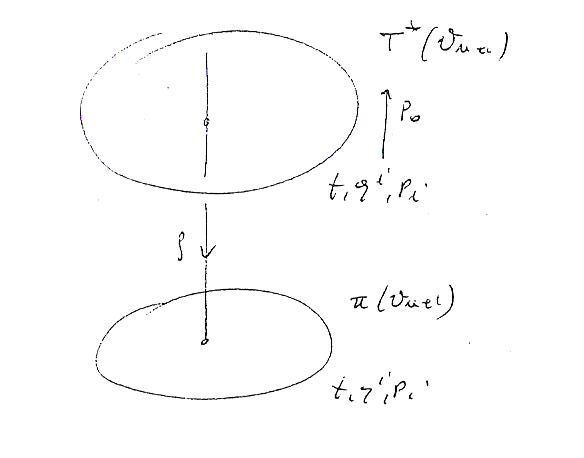
\includegraphics[width=0.5\columnwidth]{media/spazio-tempo-delle-fasi-e-struttura-di-poisson-di-tale-spazio/25-1.jpg}
\end{center}

$\pi (\mathcal{V}_{n+1})$ risulta essere una varietà differenziabile $2n+1$ dimensionale, riferita a coordinate \textit{naturali} $ t, q^i, P_i $, soggette alle leggi di trasformazione

\begin{equation*}
\begin{split}
& t' = t  \\
& q'^i = q'^i (t, q) \qquad q^i = q^i (t, q') \\
&P'_i = P_r \frac{\partial q^r}{\partial q'^i} \\
\end{split}
\end{equation*}

Una funzione $ f : \pi (\mathcal{V}_{n+1}) \rightarrow \mathbb{R} $ ($ f = f (t, q^i, P_i) $) dà luogo a una funzione $ f \circ \rho : T^* (\mathcal{V}_{n+1}) \rightarrow \mathbb{R} $ ($ f \circ \rho $ ancora descritta nella forma $ f = f (t, q^i, P_i) $). Viceversa, una funzione $ f $ definita sullo spazio $T^* (\mathcal{V}_{n+1}) $  può essere riguardata come il pull-back (attraverso $\rho$) di una funzione definita su $\pi(\mathcal{V}_{n+1})$, se e solo se $ f $ è costante lungo le fibre di $ \rho : T^* (\mathcal{V}_{n+1}) \rightarrow \pi (\mathcal{V}_{n+1}) $ ovvero se

\begin{equation} \label{eq:spazio-tempo_fasi_1}
\frac{\partial f}{\partial P_0} = 0 \qquad \Leftrightarrow \qquad \left\lbrace f, t \right\rbrace = 0
\end{equation}

si verifica facilmente che date due funzioni $ f, g $ costanti lungo le fibre di $ \rho : T^*(\mathcal{V}_{n+1}) \rightarrow \pi(\mathcal{V}_{n+1}) $, le loro parentesi di Poisson (ovviamente in $ T^* (\mathcal{V}_{n+1}) $) risulta indipendente da $ P_0 $: \\
infatti la condizione $\frac{\partial \left\lbrace f, g \right\rbrace }{\partial P_{0}} = 0$ equivale a $\left\lbrace \left\lbrace f, g \right\rbrace, t \right\rbrace = 0 $ (vedi ($ \ref{eq:spazio-tempo_fasi_1} $)) ma, per l'identità di Jacobi

\begin{equation}
\left\lbrace \left\lbrace f,g \right\rbrace ,t \right\rbrace = \left\lbrace f, \left\lbrace g,t \right\rbrace \right\rbrace - \left\lbrace g,\left\lbrace t,f \right\rbrace \right\rbrace 
\end{equation}
si ha che $ \left\lbrace g,t \right\rbrace=0$ e $\left\lbrace f,t \right\rbrace=0$ ($\Leftrightarrow \frac{\partial g}{\partial P_{0}} = 0 \text{ e } \frac{\partial f}{\partial P_{0}} = 0$) da cui la conclusione.\\
Pertanto è possibile definire operazione di \textit{parentesi di Poisson} in \textit{$\pi(\mathcal{V}_{n+1})$}
\begin{equation}
\left\lbrace f, g \right\rbrace = \frac{\partial f}{\partial q^i}\frac{\partial g}{\partial P_i}- \frac{\partial f}{\partial P_i}\frac{\partial f}{\partial q^i} \qquad \forall f, g \in \mathcal{F}(\pi (\mathcal{V}_{n+1}))
\end{equation}
Notare che $\pi (\mathcal{V}_{n+1})$ \textit{non} è una varietà simplettica (ad esempio perchè ha dimensione dispari), quindi l'esistenza di una parentesi di Poisson in $\pi (\mathcal{V}_{n+1})$ risulta un fatto non banale, e, come vedremo, molto importante.

